\section{Umformungen}
 \begin{multicols}{2}
	\subsection{Serielle Systeme}
		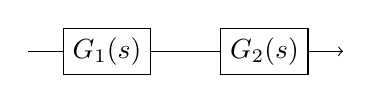
\begin{tikzpicture}
  \node (G1) at (1,0) [draw]{$G_1(s)$};

  \node (G2) at (3,0) [draw]{$G_2(s)$};

  \draw [->] (0,0) --  (node cs:name=G1) --  (node cs:name=G2)  -- ++(1,0);
\end{tikzpicture}


		$G(s) = G_1(s) \cdot G_2(s)$
	\subsection{Parallele Systeme}
		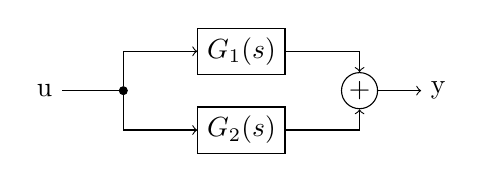
\begin{tikzpicture}
  \node (in) at (0,1) []{u};
  \node (dot) at (1,1) [draw,circle,inner sep=1,fill]{};

  \node (G1) at (2.5,1.5) [draw]{$G_1(s)$};
  \node (G2) at (2.5,0.5) [draw]{$G_2(s)$};

  \node (sum) at (4,1) [circle,draw, inner sep=1]{+};
  \node (out) at (5,1) []{y};


  \draw (in) -> (dot);
 
  \draw[->] (dot) |-  (G1);
  \draw[->] (G1) -| (sum);

  \draw[->] (dot) |-  (G2);
  \draw[->] (G2) -| (sum);

  \draw[->](sum) -- (out);

\end{tikzpicture}


		$G(s) = G_1(s) + G_2(s)$
	\subsection{Zwei Systeme mit Rückkopplung}
		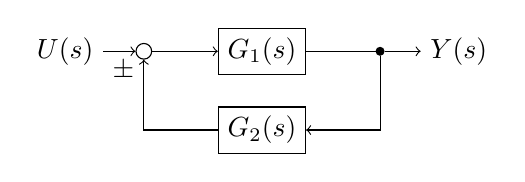
\begin{tikzpicture}
  \node (in) at (0,2) []{$U(s)$};
  \node (sum) at (1,2) [circle,draw,inner sep=2]{};
  \node (G1) at (2.5,2) [draw]{$G_1(s)$};
  \node (G2) at (2.5,1) [draw]{$G_2(s)$};
  \node (dot) at (4,2) [draw,circle,inner sep=1,fill]{};
  \node (out) at (5,2) []{$Y(s)$};

  \node (feedback) at (sum) [below left] {$\pm$};

  \draw[->] (in) -- (sum);
  \draw[->] (sum) --  (G1);
  \draw (G1) --  (dot);
  \draw[->](dot) -- (out);

  \draw[->] (dot) |-(G2);
  \draw[->] (G2) -| (sum);

\end{tikzpicture}
\newline
		$G(s) = \frac{G_1(s)}{1 \mp G_1(s) G_2(s)}$ Vorzeichenwechsel! \\
		
		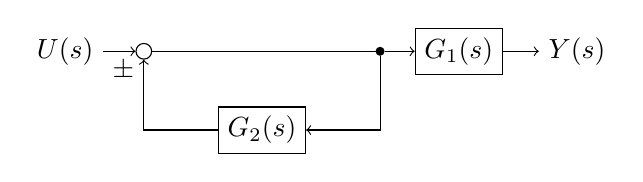
\begin{tikzpicture}
  \node (in) at (0,2) []{$U(s)$};
  \node (sum) at (1,2) [circle,draw,inner sep=2]{};
  \node (G1) at (5,2) [draw]{$G_1(s)$};
  \node (G2) at (2.5,1) [draw]{$G_2(s)$};
  \node (dot) at (4,2) [draw,circle,inner sep=1,fill]{};
  \node (out) at (6.5,2) []{$Y(s)$};

  \node (feedback) at (sum) [below left] {$\pm$};

  \draw[->] (in) -- (sum);
  \draw (sum) --  (dot);
  \draw[->] (dot) --  (G1);
  \draw[->](G1) -- (out);

  \draw[->] (dot) |-(G2);
  \draw[->] (G2) -| (sum);

\end{tikzpicture}
\newline
		$G(s) = G_1(s) \cdot \frac{1}{1 \mp G_2(s)}$ Vorzeichenwechsel!
		
  \end{multicols}
	\subsection{Komplexeres Beispiel}
		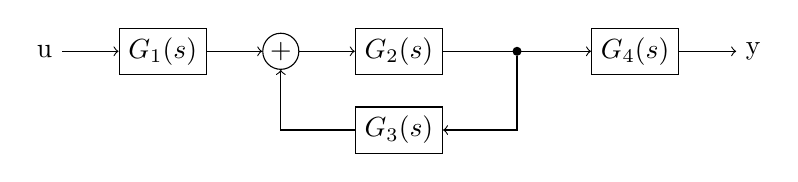
\begin{tikzpicture}
  \node (in) at (0,2) []{u};
  \node (G1) at (1.5,2) [draw]{$G_1(s)$};

  \node (sum) at (3,2) [circle,draw,inner sep=1]{+};

  \node (G2) at (4.5,2) [draw]{$G_2(s)$};
  \node (G3) at (4.5,1) [draw]{$G_3(s)$};

  \node (dot) at (6,2) [draw,circle,inner sep=1,fill]{};
  \node (G4) at (7.5,2) [draw]{$G_4(s)$};
  \node (out) at (9,2) []{y};


  \draw[->] (in) -- (G1);
 
  \draw[->] (G1) --  (sum);
  \draw[->] (sum) --  (G2);

  \draw (G2) -- (dot);
  \draw[->] (dot) |-(G3);
  \draw[->] (G3) -| (sum);

  \draw[->] (dot) |-  (G4);
  \draw[->](G4) -- (out);

\end{tikzpicture}


		$G(s) = G_1(s) \cdot \frac{G_2(s)}{1-G_2(s) \cdot G_3(s)} \cdot G_4(s)$
